\chapter{Introduction} \label{ch:introduction}

\section{Concept and Motivation}
% What are we trying to get done here?
Humanoid robots are great, and we want to get things done with them.
We ended up doing navigation and crawling.
% Navigating a humanoid robot.
Navigating a humanoid is necessary if we want to get the robot to do things
that aren't where it already is.
Get there to manipulate, create a map of environment, survey, etc.
% Crawling a humanoid robot.
Crawling can give the robot access to places where it can't walk.
Crawling is more stable.
Crawling can get you under things.
Crawling can get you over difficult terrain.
% Why are we trying to get these things done?
% Navigating is a fundamental thing for mobile robots.
% Crawling gives the robot another mode of locomotion and allows it to get to
% more places.

\begin{figure}[h!]
	\centering
    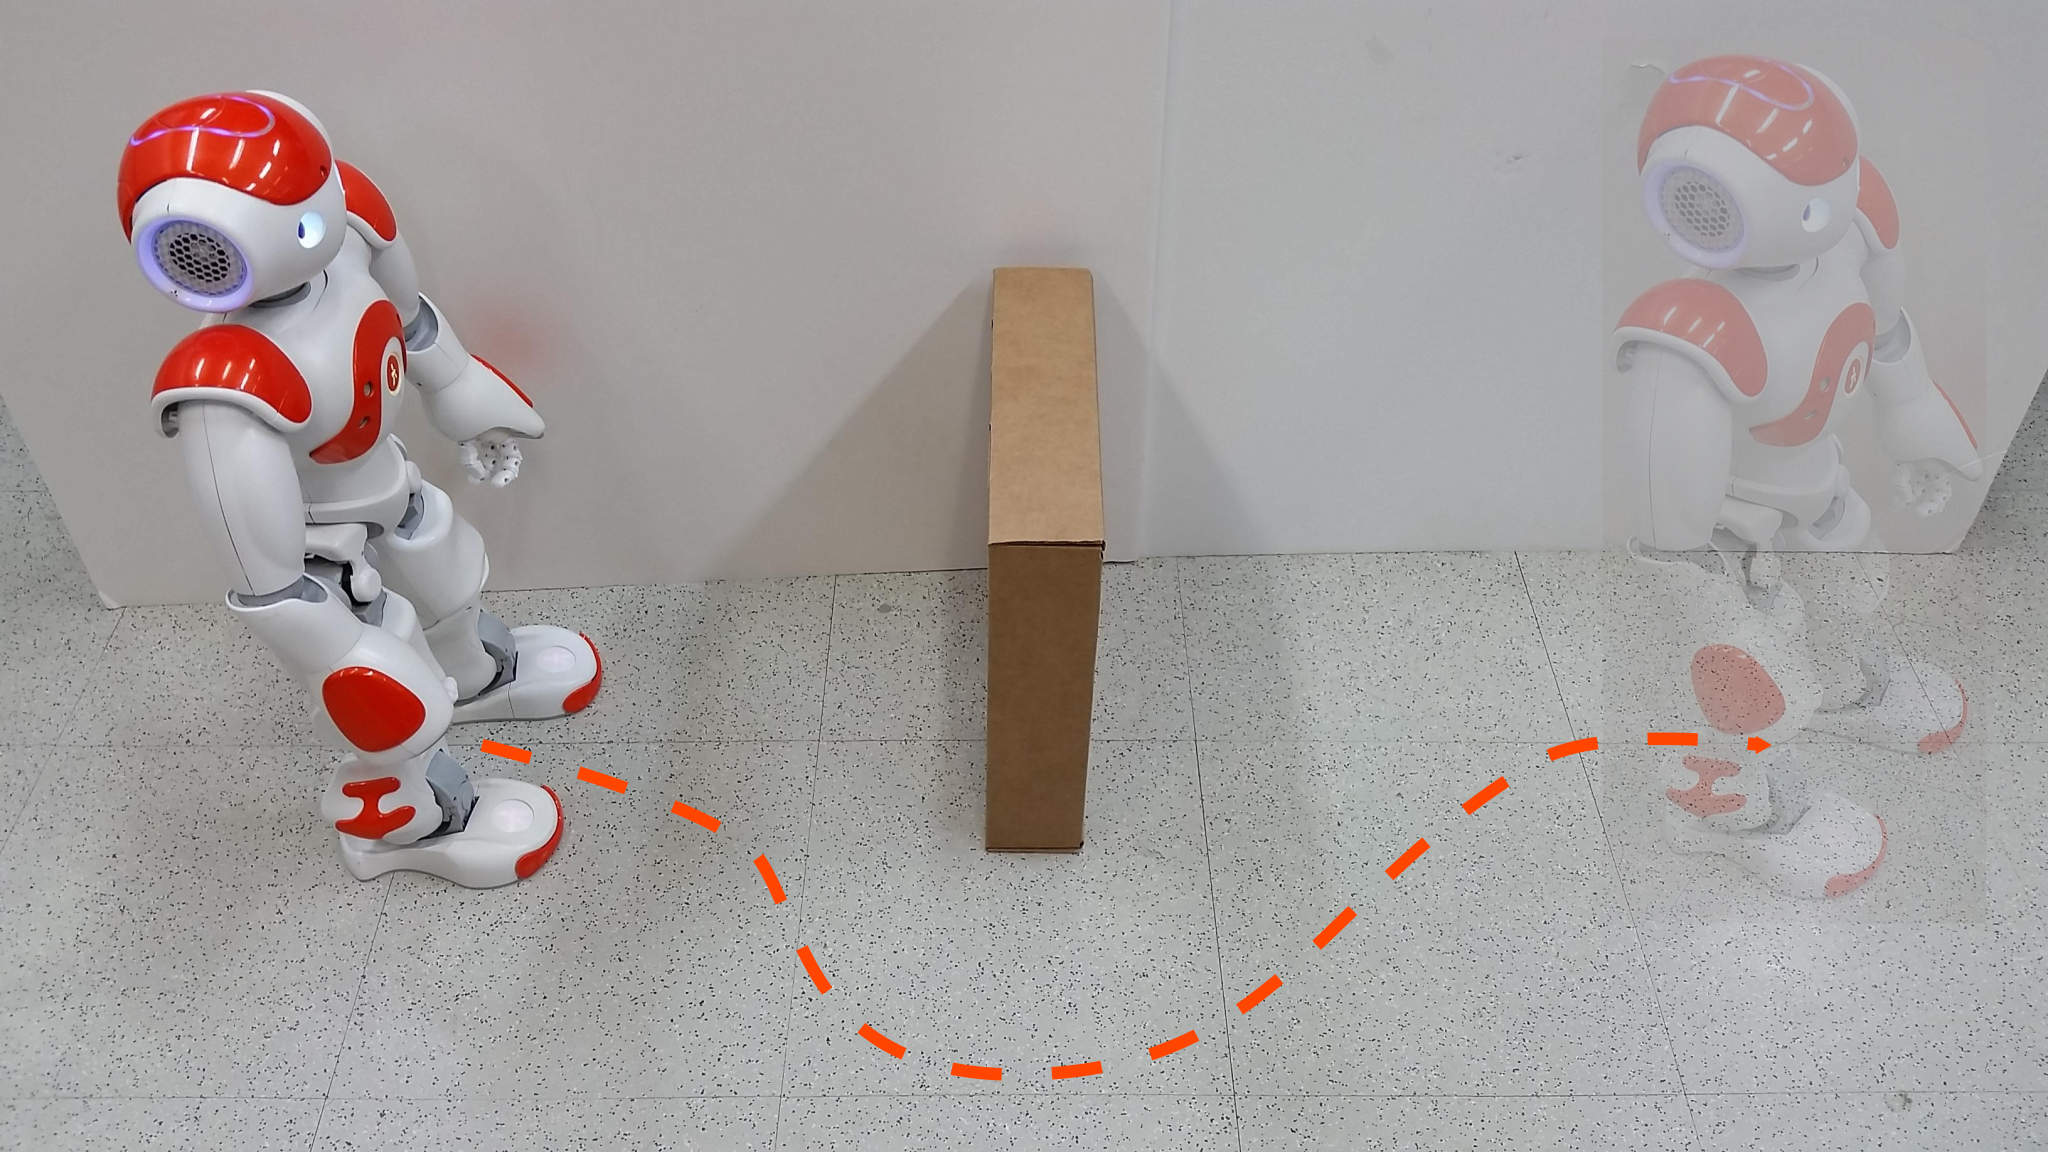
\includegraphics[width=0.7\textwidth]{nao_with_obstacle2.pdf}
	\caption{Example illustration of the Nao humanoid robot in an environment 
             with an obstacle. The red X represents a goal location with the 
             blue arrows showing an possible path. On the left side is one 
             possible representation of the environment as a 2D grid.}
	\label{fig:nao_with_obstacle2}
\end{figure}

\section{Background}
% Review previous work here as well.
% Why humanoids?
% Humanoid platforms are very adaptable. Various terrains. 
% Humanoids can locomote and manipulate.
% Humanoids are compatible with our humanoid orient environment.
% People relate to humanoids.
Humanoid robots offer a number of attractive features and interesting
challenges.
They range in size from the size of children \cite{Ishida2003, Ha2011,
Gouaillier2009, Tsagarakis2007iCubTD}, to the size of an average
adult \cite{asimo_website, atlas_website, robonaut_website, Radford2015}.
As a legged platform, it has a configuration that is adaptable 
to various terrains \cite{Iida2010, Wu2010, Lutz2012}, 
while using a minimal number of limbs to accomplish locomotion. 
In addition to being a mobile base, humanoids are also manipulators. 
This opens up possibilities for interesting interactions
with the environment \cite{levine2016, Koval2015, coleman2015}.
Humanoid platforms are also a good choice for experimenting with robots that
are expected to operate in human oriented environments as 
homes and offices are already configured to be traversable by humans.
This is showcased by competitions such as the DARPA Robotics Challenge
\cite{drc_website} and the RoboCup@Home Competitions
\cite{robocupathome_website} which both aim to further the field of robotics
toward operating in human oriented environments.
As well as being useful for navigation and manipulation, humanoid platforms
are perhaps uniquely suited for studying interactions between robots and
humans \cite{Ismail2012, Moshkina2011}. They allow for increased control
of an experiment and ensure a greater about of repeatability between
experiments.

%%% NAVIGATION %%%
% What is the problem of navigating, briefly.
% Navigation is fundamental. Get the robot somewhere safely. Otherwise it might
% as well not be mobile.
% Layered approach.
Moving a robot from one location to another in central to the problem of
mobile robotics. Navigating a mobile robot is typically implemented using
multiple approaches addressing different aspects of the problem.
% Who's done navigation?
Search-based planners, such as A* search \cite{Hart1968, gonzalez2011search,
Likhachev04ara} and Rapidly Exploring Random Trees \cite{Lavalle98rapidly} are
typically used to efficiently address global path planning, but often produce
unsmooth paths.
Planners which consider a continuous function space such as the Potential Field
algorithm \cite{ArambulaCosio2004, Koren1991, Hogan1984, Fox1997} or
Backstepping approaches \cite{Park2011, Park2015} produce smooth paths but can
have problems with complicated environments.
% We've done navigation.
The navigation algorithm used in this thesis was based on a Potential Field
approach \cite{Krishnamurthy2007}, with which we have previous experience
\cite{Brooks2013}.

%%% CRAWLING %%%
Humanoid robots have been used as a platform for exploring walking
\cite{Vukobratovic1969, Geijtenbeek2013, Deits2014}, which is important for the
field of mobile human robots. Equally important is the ability to have multiple
gaiting strategies available to traversing difficult terrain.
Humanoid crawling has been explored before in \cite{Li2011, Li_crawlingposture, 
righetti2006} and provides an interesting opportunity to expand the set of
feasible humanoid gaits \cite{Brooks2015}.

\section{Platform Overview}

\begin{figure}
	\centering
	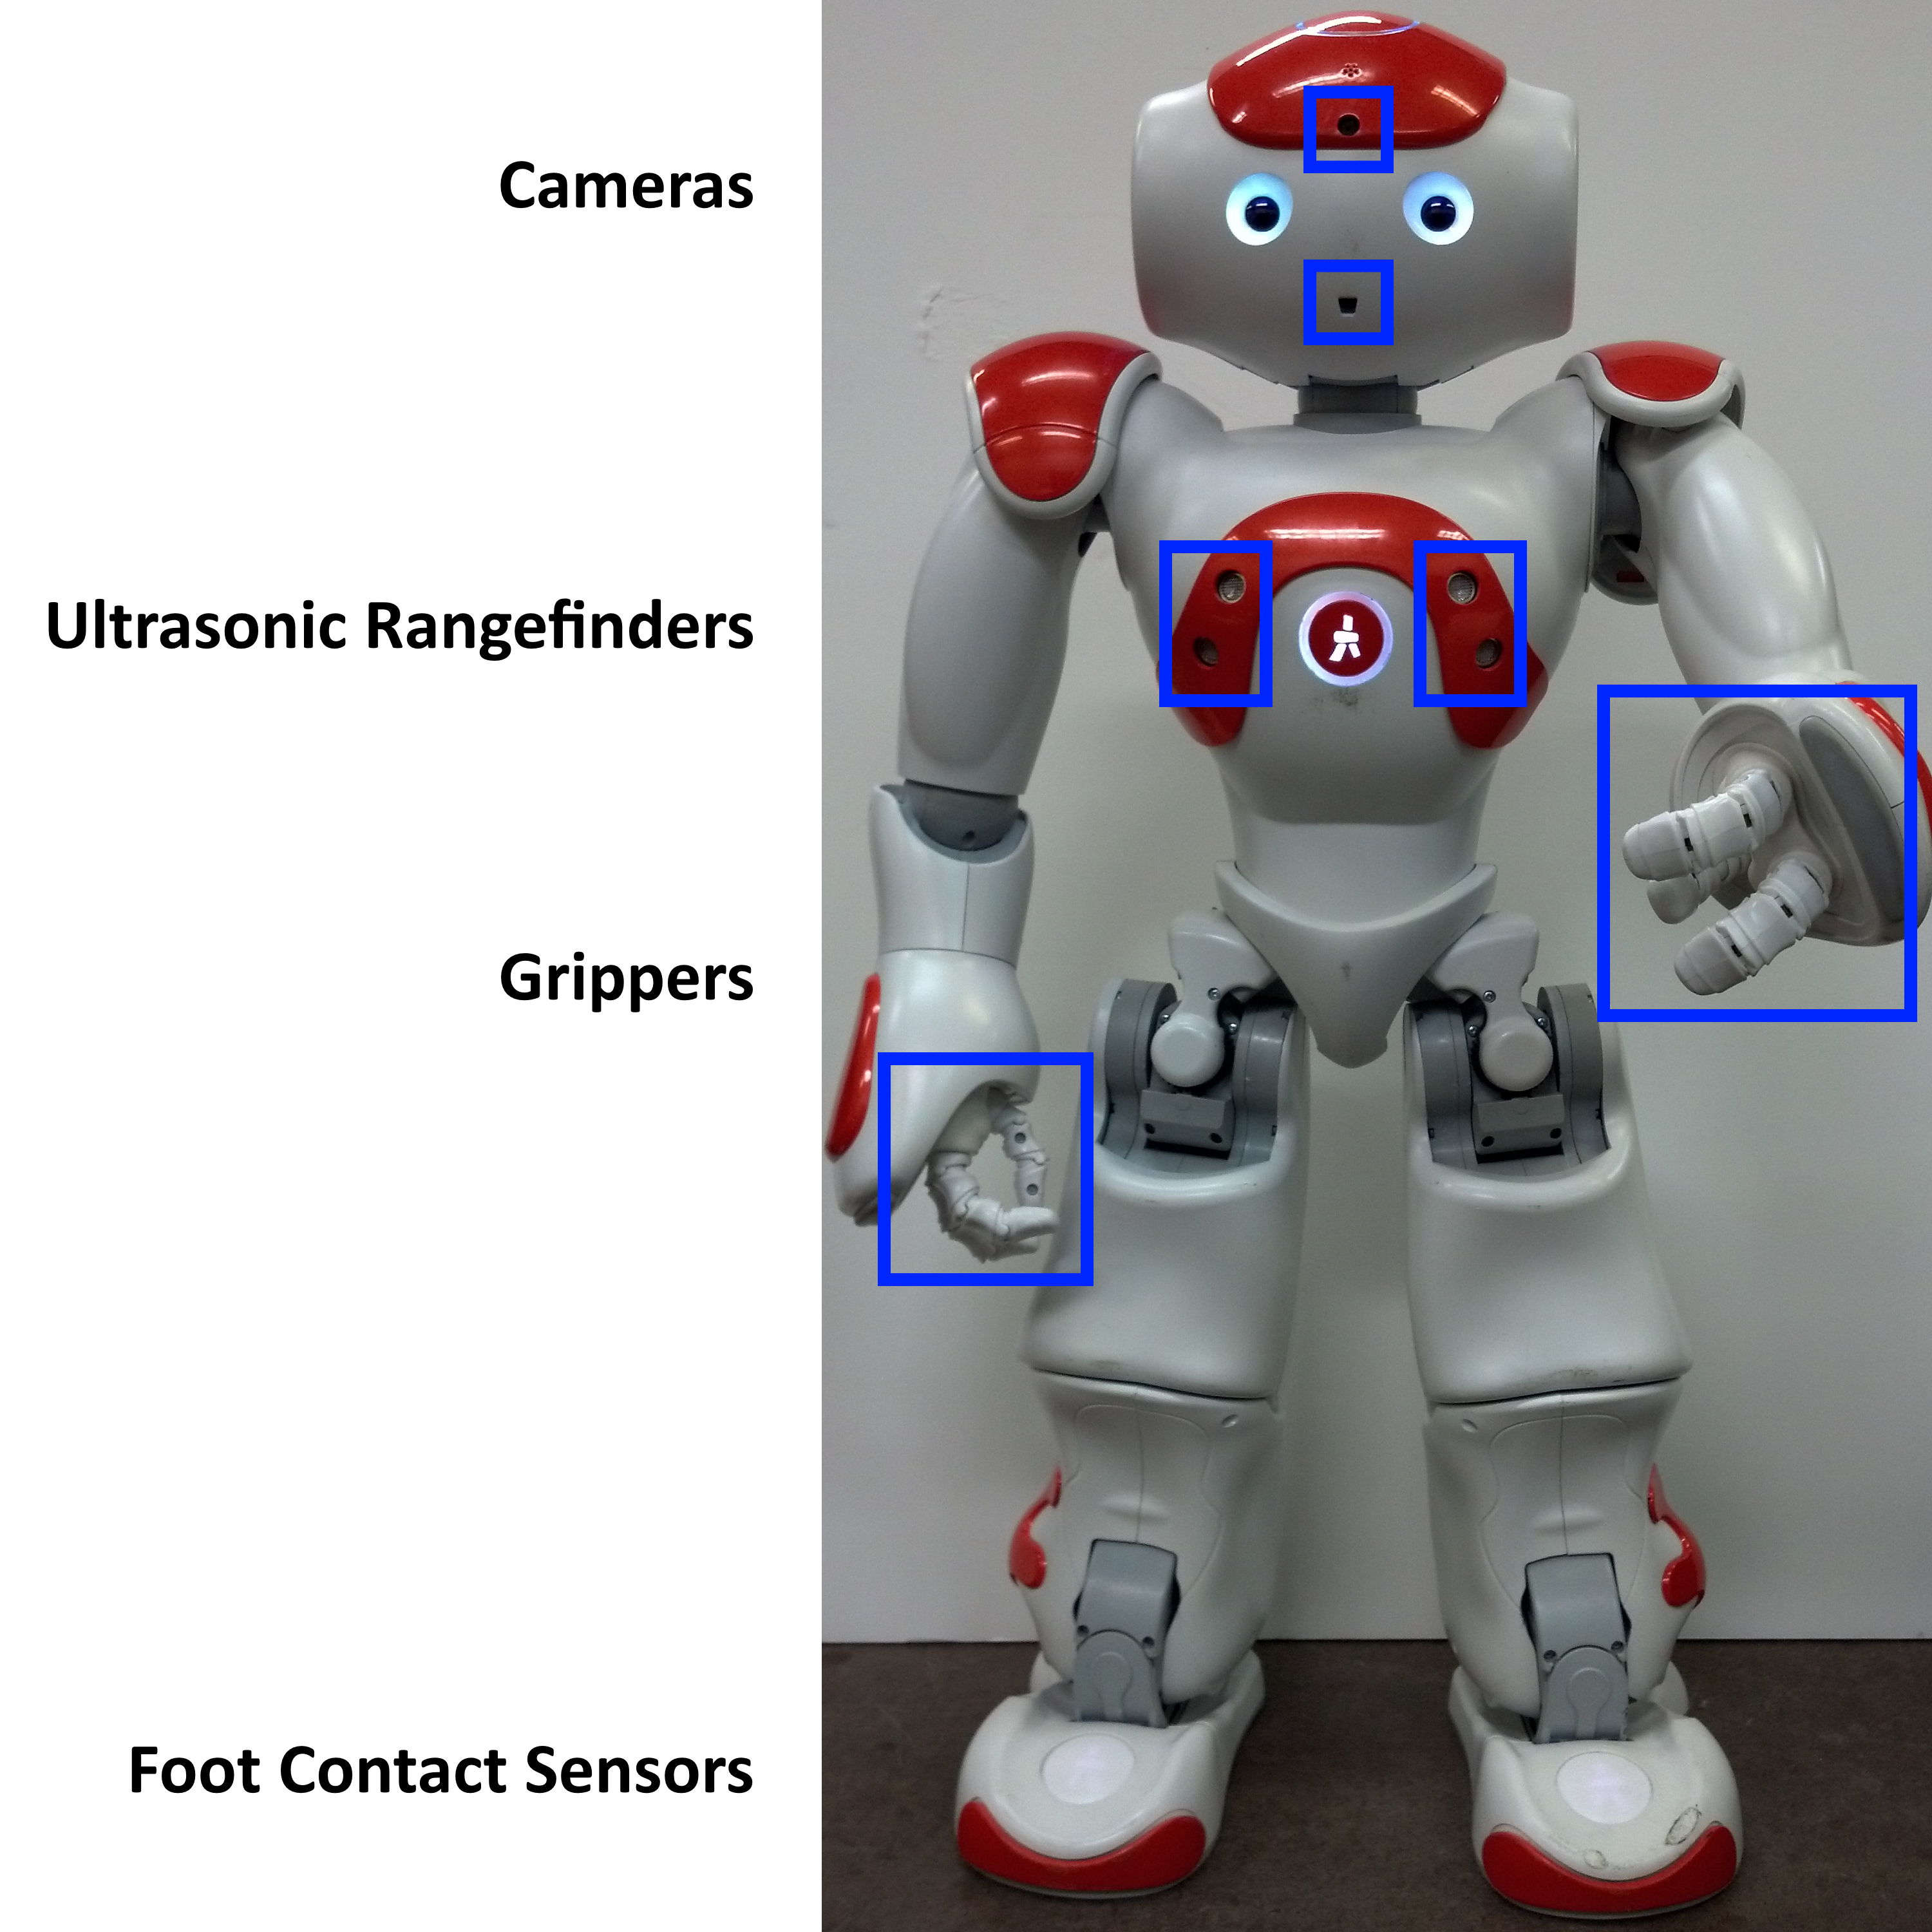
\includegraphics[width=0.4\textwidth]{nao_coronal_highlighted2.png}
    \caption{Coronal view of the Nao humanoid with a few pertinent features 
             highlighted.}
	\label{fig:nao_diagram1}
\end{figure}

% What equipment did we use?
% - Nao
% - Lidar
% - Mount
We used a Nao. What's that?
We used a Lidar. What's that? We used a Hokuyo. What's that?
We made a mount.

% Why did we use these things?
We used a Nao, because it's a humanoid.
We used a Lidar because you can see more things.
We had to make a mount to get it on there.


\section{GODZILA Navigation}
% Briefly, what's navigation?
% What approach did we go for?
% Why did we go for this?
GODZILA is a potential field local approach.
Potential field is this blah.
It's cheap on memory and fast to compute.
It's local. Now we can build more on top of it.

\section{Projected Profile Crawl Gait}
% Briefly, what's crawling?
% Why crawling?
% What approach did we go for?
% Why did we go for this approach?
Statically stable.
You take the robot as symmetric and do a saggital projection.
Can compose the gait into two modes.
Applicable to other platforms.

\section{Thesis Structure}
This thesis is organized as follows: 

% Chapter \ref{ch:platform} reviews the Nao Humanoid Platform with Hokoyu Scanning Laser Rangefinder augmentation.
% The navigation system is broken into three parts, 
% Chapter \ref{ch:navigation} discusses the GODZILA algorithm used for local navigation.
% Chapter \ref{ch:crawl_gait} discusses the Projected Profile crawling gait used to perform the crawl.
% Simulations and experimental results are shown in Chapters \ref{ch:simulations} and \ref{ch:results}, 
% while a discussion of the work is given in Chapter \ref{ch:conclusion}.
